\documentclass[11pt,letterpaper]{article}

% ============================================================
% PAQUETES
% ============================================================
\usepackage[utf8]{inputenc}
\usepackage[T1]{fontenc}
\usepackage[spanish,es-noindentfirst,es-tabla]{babel}
\decimalpoint
\usepackage[margin=2.5cm]{geometry}
\usepackage{graphicx}
\usepackage{booktabs}
\usepackage{array}
\usepackage{multirow}
\usepackage{siunitx}
\sisetup{output-decimal-marker={.}, group-digits=false, detect-weight=true, table-number-alignment=center}
\usepackage{amsmath,amssymb}
\usepackage{listings}
\usepackage{xcolor}
\usepackage{fancyhdr}
\usepackage{titlesec}
\usepackage{caption}
\usepackage[section]{placeins}
\usepackage[hidelinks]{hyperref}

\graphicspath{{figuras/}}
\renewcommand{\topfraction}{0.92}
\renewcommand{\bottomfraction}{0.85}
\renewcommand{\textfraction}{0.06}
\renewcommand{\floatpagefraction}{0.80}
\setcounter{topnumber}{3}
\setcounter{totalnumber}{5}
\makeatletter
\setlength{\@fptop}{0pt}
\setlength{\@fpsep}{12pt}
\makeatother
\captionsetup{font=small,labelfont=bf}

% ============================================================
% ESTILO DE CÓDIGO
% ============================================================
\lstdefinestyle{codigo}{
    basicstyle=\ttfamily\footnotesize,
    keywordstyle=\color{blue!60!black}\bfseries,
    commentstyle=\color{gray},
    stringstyle=\color{orange!70!black},
    numbers=left,
    numberstyle=\tiny\color{gray},
    frame=single,
    breaklines=true,
    showstringspaces=false,
    tabsize=2,
    backgroundcolor=\color{gray!5},
    extendedchars=true,
    columns=fullflexible,
    keepspaces=true,
    upquote=true,
    literate={á}{{\'a}}1 {é}{{\'e}}1 {í}{{\'i}}1 {ó}{{\'o}}1 {ú}{{\'u}}1
             {Á}{{\'A}}1 {É}{{\'E}}1 {Í}{{\'I}}1 {Ó}{{\'O}}1 {Ú}{{\'U}}1
             {ñ}{{\~n}}1 {Ñ}{{\~N}}1 {¿}{{?`}}1 {¡}{{!`}}1
}
\lstset{style=codigo}

% ============================================================
% ENCABEZADO / PIE DE PÁGINA
% ============================================================
\pagestyle{fancy}
\fancyhf{}
\lhead{Taller 2 --- MLP y Backpropagation}
\rhead{Inteligencia Computacional Aplicada}
\cfoot{\thepage}
\renewcommand{\headrulewidth}{0.4pt}

\titleformat{\section}{\normalfont\Large\bfseries}{\thesection.}{0.5em}{}
\titleformat{\subsection}{\normalfont\large\bfseries}{\thesubsection}{0.5em}{}

% ============================================================
% DATOS DEL INFORME
% ============================================================
\newcommand{\nombreEstudiante}{Sergio Santiago Duarte Rojas}
\newcommand{\codigoEstudiante}{20261595002}
\newcommand{\nombreDocente}{Cesar Andrey Perdomo Charry}
\newcommand{\nombreAsignatura}{Inteligencia Computacional Aplicada}
\newcommand{\fechaInforme}{\today}

\begin{document}

% ============================================================
% PORTADA
% ============================================================
\begin{titlepage}
    \centering
    \vspace*{2cm}
    {\LARGE \bfseries Taller 2: Redes Neuronales Multicapa (MLP)\\ y Backpropagation\par}
    \vspace{0.5cm}
    {\large Informe de Resultados\par}
    \vspace{2cm}

    \begin{tabular}{ll}
        \textbf{Asignatura:} & \nombreAsignatura \\
        \textbf{Docente:}    & \nombreDocente \\
        \textbf{Estudiante:} & \nombreEstudiante \\
        \textbf{Código:}     & \codigoEstudiante \\
        \textbf{Fecha:}      & \fechaInforme \\
    \end{tabular}

    \vfill
    Universidad Distrital Francisco José de Caldas
\end{titlepage}

\tableofcontents
\newpage

% ============================================================
\section{Introducción}

El Perceptrón y el Adaline del Taller 1 no pudieron con la XOR, porque una neurona traza un solo hiperplano y la XOR necesita dos. Este taller implementa un perceptrón multicapa entrenado por retropropagación y comprueba qué gana la red al agregar la capa oculta.

Se completaron las cuatro funciones pendientes del \textit{live script} del docente sin cambiar nombres ni argumentos, y sobre ellas se montaron los experimentos de los numerales 3 a 6. La XOR de dos y tres entradas se compara con el Taller 1 y sobre ella se estudian el barrido de tasa y momento de la guía de laboratorio (2007), la escala de los pesos iniciales y la activación de cada capa. Iris se prueba con cuatro arquitecturas y tres tasas. Wine, Breast Cancer Wisconsin y billetes se evalúan en cuatro particiones frente al Perceptrón y el Adaline, y en Breast Cancer se analiza el sobreajuste y la parada temprana que lo corrige.

% ============================================================
\section{Marco teórico (resumen)}

\subsection{Arquitectura del perceptrón multicapa}

Un perceptrón multicapa organiza las neuronas en capas sucesivas. La capa de entrada solo distribuye el patrón, cada capa oculta calcula una suma ponderada de las salidas de la capa anterior y le aplica una función de activación, y la capa de salida entrega la respuesta de la red. Para la neurona $j$ de la capa $k$ el cálculo es el de la ecuación \eqref{eq:forward}, donde $a^{(0)}$ es la entrada $x$.
\begin{equation}
    net_j^{(k)} = \sum_i w_{ji}^{(k)} a_i^{(k-1)} + b_j^{(k)}, \qquad a_j^{(k)} = f\left(net_j^{(k)}\right)
    \label{eq:forward}
\end{equation}
Este recorrido desde la entrada hasta la salida se llama propagación hacia adelante. La diferencia con la neurona única del Taller 1 está en que la función $f$ de las capas ocultas debe ser derivable y no lineal, con la salvedad de la ReLU, que no es derivable en cero y a la que ahí se le asigna derivada cero. El taller ofrece tres opciones, la sigmoide $1/(1+e^{-net})$ que produce valores entre cero y uno, la tangente hiperbólica que produce valores entre menos uno y uno, y la ReLU, que vale $net$ cuando es positivo y cero en caso contrario.

\subsection{El algoritmo de retropropagación}
\label{sec:backprop}

La red se entrena minimizando el error cuadrático $E = \tfrac{1}{2}\sum (d(x) - Y(x))^2$ por descenso de gradiente, igual que el Adaline. La novedad es que ahora hay pesos en capas que no ven directamente el error, y para corregirlos hace falta repartir ese error hacia atrás. El reparto se hace con un término $\delta$ por neurona. En la capa de salida el término se calcula con el error observado, ecuación \eqref{eq:delta_out}, y en cada capa oculta se obtiene a partir de los $\delta$ de la capa siguiente pesados por las conexiones que las unen, ecuación \eqref{eq:delta_hid}, donde $\odot$ es el producto elemento a elemento y $W^{T}$ la traspuesta de la matriz de pesos.
\begin{align}
    \delta^{(L)} &= \left(d(x) - Y(x)\right) \odot f'\left(net^{(L)}\right) \label{eq:delta_out} \\
    \delta^{(k)} &= \left(W^{(k+1)T}\delta^{(k+1)}\right) \odot f'\left(net^{(k)}\right) \label{eq:delta_hid}
\end{align}
Con los $\delta$ calculados, cada peso se corrige en proporción al $\delta$ de la neurona que alimenta y a la activación que recibe, ecuación \eqref{eq:update}, donde $\eta$ es la tasa de aprendizaje. El coeficiente de momento $\beta$, que la guía de laboratorio del curso (2007) propone variar entre 0 y 1, agrega una fracción del incremento anterior, lo cual acelera el avance cuando los incrementos sucesivos apuntan en la misma dirección.
\begin{equation}
    \Delta W^{(k)} = \eta\, \delta^{(k)} \left(a^{(k-1)}\right)^T + \beta\, \Delta W^{(k)}_{\text{anterior}}, \qquad W^{(k)} \leftarrow W^{(k)} + \Delta W^{(k)}
    \label{eq:update}
\end{equation}
Cuando la red tiene una sola capa y activación lineal, las ecuaciones \eqref{eq:delta_out} y \eqref{eq:update} se reducen a la Regla Delta del Taller 1. La retropropagación es entonces la extensión natural de ese algoritmo a redes con capas ocultas.

\subsection{Por qué la XOR necesita una capa oculta}

Una neurona con función escalón divide el espacio de entrada en dos regiones separadas por un hiperplano. La XOR asigna la clase uno a $(0,1)$ y $(1,0)$ y la clase cero a $(0,0)$ y $(1,1)$, y ninguna recta deja a cada lado los puntos de una clase. Con una capa oculta la red traza dos rectas y las combina. Dos neuronas ocultas bastan en principio, una que se activa cuando alguna entrada vale uno y otra cuando ambas valen uno, y la salida responde uno solo cuando la primera está activa y la segunda no. Rumelhart, Hinton y Williams (1986) mostraron que una capa oculta entrenada por retropropagación resuelve exactamente este tipo de problema.

\subsection{Sobreajuste y parada temprana}

Una red con suficientes pesos y épocas puede aprender de memoria los datos de entrenamiento. El síntoma es que el error de entrenamiento sigue bajando mientras el error sobre datos no vistos deja de bajar y sube. Eso es el sobreajuste (Haykin, 2009). La parada temprana vigila el error sobre un conjunto de validación y detiene el entrenamiento cuando lleva cierto número de épocas sin mejorar, conservando los pesos del mejor punto. Es el criterio de parada por épocas sin mejora que pide el numeral 2.

% ============================================================
\section{Metodología}

\subsection{Implementación}

\texttt{init\_mlp} crea pesos aleatorios pequeños y sesgos en cero. \texttt{forward\_mlp} aplica la ecuación \eqref{eq:forward} capa por capa y guarda las sumas ponderadas y las activaciones. \texttt{backward\_mlp} calcula los $\delta$ de las ecuaciones \eqref{eq:delta_out} y \eqref{eq:delta_hid} y actualiza pesos y sesgos con la ecuación \eqref{eq:update}. \texttt{activation\_deriv} entrega la derivada de cada activación. La activación oculta se indica con un nombre para todas las capas o con una lista con una por capa. La plantilla usaba \texttt{net} sin haberla creado, así que se agregó la llamada a \texttt{init\_mlp}. El código va en el Anexo \ref{anexo:codigo}.

\texttt{train\_mlp} repite el ciclo de la plantilla, calcula en cada época el error de validación e implementa la parada por épocas sin mejora con el campo \texttt{patience}. Las demás funciones predicen la clase, cargan cada conjunto, parten con semilla y escalan al rango cero a uno, estas dos últimas tomadas del Taller 1. \texttt{Dataset\_train\_test\_T2} es la versión para Wine y Breast Cancer del script de particiones del Taller 1, con la misma semilla que el experimento. El Perceptrón y el Adaline se incluyen sin cambios, y con más de dos clases se entrena una neurona por clase y decide la mayor suma ponderada.

\subsection{Arquitecturas y parámetros evaluados}

La Tabla \ref{tab:config} recoge las configuraciones. Salvo donde se indica, se usan salida sigmoide, pesos iniciales de escala 0.5, tasa 0.3 y el error objetivo de la plantilla, 0.001. En las compuertas cada configuración se repite con cinco semillas. Las arquitecturas entre corchetes tienen dos capas ocultas. El Perceptrón y el Adaline conservan los parámetros del Taller 1, tasa 0.1 y 100 épocas el primero, tasa 0.05 y 200 épocas el segundo. Las tablas y figuras llaman MSE al error $E$ de la sección \ref{sec:backprop} promediado sobre los patrones.

\begin{table}[!htb]
    \centering
    \caption{Configuraciones de MLP evaluadas. La parada es por error objetivo o por número de épocas sin mejora en validación}
    \label{tab:config}
    \scriptsize
    \setlength{\tabcolsep}{3pt}
    \begin{tabular}{llcccc l}
        \toprule
        \textbf{Experimento} & \textbf{Ocultas} & \textbf{Activación oculta} & $\boldsymbol{\eta}$ & \textbf{Momento} & \textbf{Épocas} & \textbf{Parada} \\
        \midrule
        XOR & 2, 4, 8, [4 4] & sigmoide, tanh, ReLU & 0.1 a 2 & 0 a 1 & 5000 & error 0.001 \\
        Iris & 3, 6, 12, [8 4] & sigmoide & 0.05, 0.1, 0.3 & 0 & 1000 & error 0.001 \\
        Conjuntos reales & 8 & sigmoide & 0.3 & 0 & 500 & error 0.001 o 30 sin mejora \\
        Sobreajuste & 2, 8, 32, 64 & sigmoide & 0.1 & 0 & 200 a 1500 & ninguna o 50 sin mejora \\
        \bottomrule
    \end{tabular}
\end{table}

\subsection{Conjuntos de datos y particiones}

La XOR de $n$ entradas vale uno cuando un número impar de entradas vale uno, 4 patrones con dos entradas y 8 con tres. Iris tiene 150 flores, cuatro medidas y tres especies, codificadas con una salida por especie. Wine tiene 178 vinos de tres bodegas con trece medidas. Breast Cancer Wisconsin Diagnostic tiene 569 tumores con treinta medidas, 357 benignos y 212 malignos. Billetes es el conjunto del Taller 1, 1372 patrones, cuatro medidas y dos clases. Wine proviene de Aeberhard y Forina (1991), Breast Cancer de Wolberg et al. (1993) y billetes de Lohweg (2013), todos del repositorio UCI, e Iris es el conjunto de Fisher (1936). La Tabla \ref{tab:tamanos} resume los tamaños.

\begin{table}[!htb]
    \centering
    \caption{Conjuntos de datos empleados}
    \label{tab:tamanos}
    \footnotesize
    \begin{tabular}{l S[table-format=4.0] S[table-format=2.0] S[table-format=1.0] l}
        \toprule
        \textbf{Conjunto} & {\textbf{Patrones}} & {\textbf{Entradas}} & {\textbf{Clases}} & \textbf{Uso} \\
        \midrule
        XOR de 2 entradas & 4 & 2 & 2 & numeral 3 \\
        XOR de 3 entradas & 8 & 3 & 2 & numeral 3 \\
        Iris & 150 & 4 & 3 & numeral 4 \\
        Wine & 178 & 13 & 3 & numeral 5 \\
        Breast Cancer Wisconsin & 569 & 30 & 2 & numerales 5 y 6 \\
        Billetes & 1372 & 4 & 2 & numeral 5 \\
        \bottomrule
    \end{tabular}
\end{table}

Las particiones mezclan los índices con semilla fija y cortan en 60-40, 70-30, 80-20 y 90-10, como en el Taller 1. Las entradas se escalan al rango cero a uno con los mínimos y máximos del entrenamiento. Cuando hace falta validación, para la curva de error o para la parada temprana, se aparta una quinta parte del entrenamiento con una segunda semilla, y la exactitud se mide siempre sobre un conjunto de prueba que la red no vio. El Perceptrón y el Adaline no usan validación y entrenan con el conjunto de entrenamiento completo.

% ============================================================
\section{Resultados}

\subsection{Problema XOR}

La Tabla \ref{tab:xor} compara los tres modelos. El Perceptrón y el Adaline no convergen en ninguna semilla y quedan en 30 por ciento con dos entradas, frente al 25 por ciento del Taller 1 con una sola semilla, y cerca del 50 con tres, el nivel de responder siempre la misma clase. El MLP con cuatro u ocho neuronas ocultas resuelve la XOR de dos entradas en todas las semillas, con entre 3443 y 4117 épocas para bajar el error por debajo de 0.001 con tasa 0.3 y sin momento. Con dos neuronas, el mínimo teórico, las cinco semillas clasifican bien pero una no alcanza el error objetivo. Con tres entradas solo la capa de ocho neuronas converge en la mayoría de las semillas, y el momento 0.9 lleva a las cinco al objetivo en ambos problemas.

\begin{table}[!htb]
    \centering
    \caption{XOR de dos y tres entradas. Promedio de cinco semillas. El Perceptrón y el Adaline usan los parámetros del Taller 1, el MLP la tasa 0.3 y el momento que indica su columna. Convergió es el porcentaje de semillas que alcanzan el error objetivo, y un promedio de 5000 épocas indica que ninguna lo alcanzó}
    \label{tab:xor}
    \footnotesize
    \begin{tabular}{llcc S[table-format=4.1] S[table-format=3.0] S[table-format=3.1]}
        \toprule
        \textbf{Entradas} & \textbf{Modelo} & \textbf{Ocultas} & \textbf{Momento} & {\textbf{Épocas}} & {\textbf{Convergió (\%)}} & {\textbf{Exactitud (\%)}} \\
        \midrule
        \multirow{6}{*}{2} & Perceptrón & ninguna & {--} & 100.0  & 0   & 30.0  \\
                           & Adaline    & ninguna & {--} & 200.0  & 0   & 30.0  \\
                           & MLP        & 2       & 0    & 4406.0 & 80  & 100.0 \\
                           & MLP        & 4       & 0    & 4116.6 & 100 & 100.0 \\
                           & MLP        & 8       & 0    & 3443.0 & 100 & 100.0 \\
                           & MLP        & 4       & 0.9  & 435.8  & 100 & 100.0 \\
        \midrule
        \multirow{6}{*}{3} & Perceptrón & ninguna & {--} & 100.0  & 0   & 47.5  \\
                           & Adaline    & ninguna & {--} & 200.0  & 0   & 50.0  \\
                           & MLP        & 2       & 0    & 5000.0 & 0   & 62.5  \\
                           & MLP        & 4       & 0    & 4187.8 & 40  & 75.0  \\
                           & MLP        & 8       & 0    & 3122.8 & 80  & 92.5  \\
                           & MLP        & 4       & 0.9  & 1231.4 & 100 & 100.0 \\
        \bottomrule
    \end{tabular}
\end{table}

La Tabla \ref{tab:xor_param} aísla el momento y la activación. Con cuatro neuronas y momento 0.9 la XOR de dos entradas converge en 436 épocas en lugar de 4117, y la de tres pasa de dos semillas convergidas a cinco. La tangente hiperbólica también acelera, 880 épocas en dos entradas, y la ReLU resulta poco fiable, tres de cinco semillas en dos entradas y ninguna en tres. La red de dos capas ocultas con tanh y sigmoide es la más rápida de esta tabla, 149 y 260 épocas, aunque como combina segunda capa, tanh y momento la tabla no permite separar cuánto aporta cada uno. La Figura \ref{fig:xor} muestra la curva de error del MLP con momento 0.9 frente a la del Adaline, que se estabiliza cerca de 0.139, apenas por encima del piso de 0.125 de la mejor función lineal, la que responde 0.5 en los cuatro patrones.

\begin{table}[!htb]
    \centering
    \caption{Efecto del momento y de la activación oculta sobre la XOR, y una red de dos capas ocultas con activación distinta en cada una. Promedio de cinco semillas, Convergió como en la Tabla \ref{tab:xor}}
    \label{tab:xor_param}
    \footnotesize
    \begin{tabular}{lclc S[table-format=4.1] S[table-format=3.0] S[table-format=3.1]}
        \toprule
        \textbf{Entradas} & \textbf{Ocultas} & \textbf{Activación oculta} & \textbf{Momento} & {\textbf{Épocas}} & {\textbf{Convergió (\%)}} & {\textbf{Exactitud (\%)}} \\
        \midrule
        \multirow{6}{*}{2} & 4     & sigmoide       & 0   & 4116.6 & 100 & 100.0 \\
                           & 4     & sigmoide       & 0.5 & 2087.6 & 100 & 100.0 \\
                           & 4     & sigmoide       & 0.9 & 435.8  & 100 & 100.0 \\
                           & 4     & tanh           & 0   & 879.8  & 100 & 100.0 \\
                           & 4     & ReLU           & 0   & 2416.4 & 60  & 90.0  \\
                           & {[4 4]} & tanh, sigmoide & 0.9 & 149.0 & 100 & 100.0 \\
        \midrule
        \multirow{6}{*}{3} & 4     & sigmoide       & 0   & 4187.8 & 40  & 75.0  \\
                           & 4     & sigmoide       & 0.5 & 4281.2 & 20  & 95.0  \\
                           & 4     & sigmoide       & 0.9 & 1231.4 & 100 & 100.0 \\
                           & 4     & tanh           & 0   & 1516.0 & 80  & 90.0  \\
                           & 4     & ReLU           & 0   & 5000.0 & 0   & 87.5  \\
                           & {[4 4]} & tanh, sigmoide & 0.9 & 259.6 & 100 & 100.0 \\
        \bottomrule
    \end{tabular}
\end{table}

\begin{figure}[!htb]
    \centering
    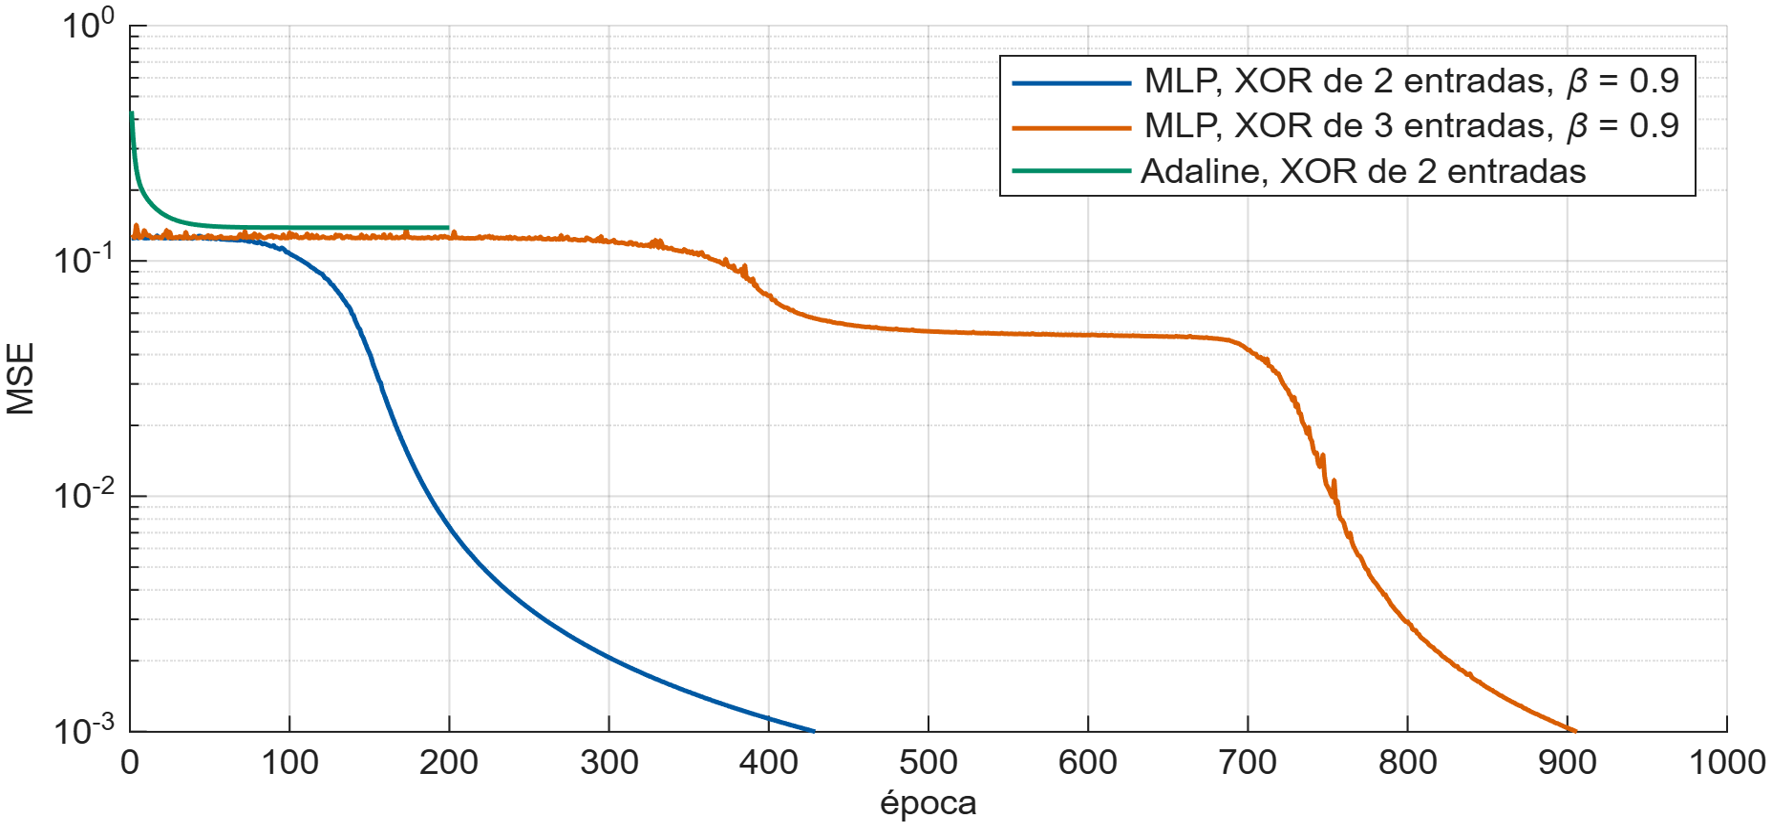
\includegraphics[width=15cm]{fig02.png}
    \caption{Curvas de error de entrenamiento sobre la XOR de dos y tres entradas con una de las cinco semillas, en escala logarítmica. El MLP con cuatro neuronas ocultas y momento 0.9 llega al error objetivo en ambos casos, y el Adaline se estanca cerca de 0.139, apenas por encima del piso de 0.125 de la mejor función lineal}
    \label{fig:xor}
\end{figure}

\subsection{Tasa de aprendizaje, momento y pesos iniciales sobre la XOR}

La guía de laboratorio del curso (2007) propone variar la tasa entre 0.1 y 2 con momento cero y el momento entre 0 y 1 con tasa 0.5. La Figura \ref{fig:barrido} reproduce ese barrido con cuatro neuronas ocultas y cinco semillas, y agrega la escala de los pesos iniciales. Con tasas 0.1 y 0.2 ninguna semilla llega al objetivo en 5000 épocas. De 0.3 en adelante todas convergen y cada vez más rápido, de 4117 épocas a 736 con tasa 2, sin que la tasa grande desestabilice el entrenamiento, porque la sigmoide acota las salidas y los cuatro patrones no tienen ruido. El momento reduce las épocas de forma sostenida, de 2565 sin momento a 266 con 0.9, y con momento 1 el incremento anterior nunca se amortigua y nadie converge.

La escala inicial tiene un rango útil estrecho. Con 0.1 las neuronas ocultas arrancan casi iguales y el error no baja del objetivo en 5000 épocas. Entre 0.5 y 2 convergen todas las semillas. Con 5 las sumas ponderadas caen en la zona plana de la sigmoide, donde la derivada $f(1-f)$ es casi cero, y solo tres de cinco semillas salen de ahí.

\begin{figure}[!htb]
    \centering
    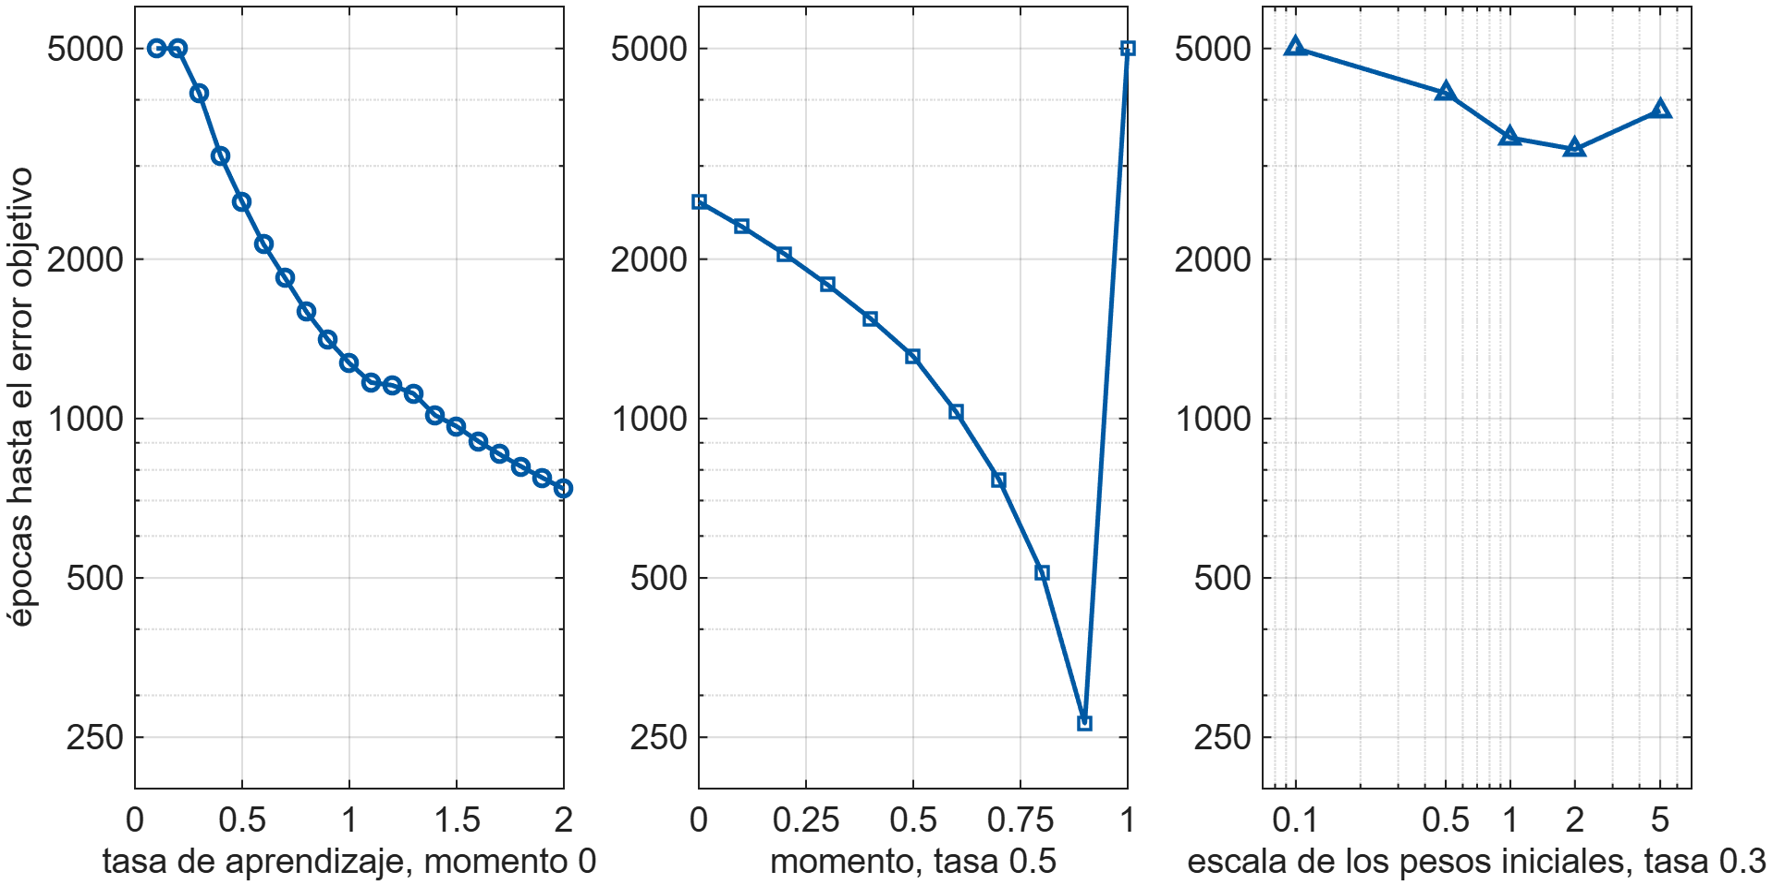
\includegraphics[width=15cm]{fig03.png}
    \caption{Épocas hasta el error objetivo sobre la XOR de dos entradas al variar la tasa de aprendizaje, el momento y la escala de los pesos iniciales, cuatro neuronas ocultas y promedio de cinco semillas. Un valor de 5000 indica que no se alcanzó el objetivo. Escala logarítmica en el eje vertical, y el tercer panel usa tasa 0.3}
    \label{fig:barrido}
\end{figure}


\subsection{Activación en la capa oculta frente a la capa de salida}

El numeral 1 pide elegir por separado la activación de las capas ocultas y la de salida, y la Tabla \ref{tab:oculta_salida} muestra qué cambia cada elección. La capa de salida fija la forma del $\delta$ de la ecuación \eqref{eq:delta_out}, con $f'$ igual a uno si es lineal y menor que uno si es sigmoide o tanh, y decide si la salida queda acotada. La capa oculta fija qué tan rápido se despega la red de la meseta inicial. En la XOR la combinación más rápida fue tanh en la oculta con salida sigmoide, 95 épocas frente a 436 de sigmoide con sigmoide, porque la tanh centrada en cero mueve más los pesos ocultos y la sigmoide de salida acota el error. Con salida tanh o lineal sobre una oculta tanh, y con salida lineal sobre una oculta ReLU, ninguna semilla llega al objetivo, porque con momento 0.9 una salida sin cota o con cuatro veces la pendiente de la sigmoide da pasos demasiado grandes y la red oscila. Con salida sigmoide, la ReLU oculta vuelve a ser la menos fiable, 60 por ciento de semillas convergidas. En Breast Cancer las nueve combinaciones quedan entre 95.3 y 97.7 por ciento, así que sobre un problema separable con datos escalados la elección pesa mucho menos que sobre la XOR.

\begin{table}[!htb]
    \centering
    \caption{Activación de la capa oculta frente a la de salida. XOR de dos entradas con cuatro neuronas ocultas, momento 0.9 y cinco semillas, y Breast Cancer 70-30 con ocho neuronas ocultas y una semilla. Convergió como en la Tabla \ref{tab:xor}}
    \label{tab:oculta_salida}
    \footnotesize
    \begin{tabular}{ll S[table-format=4.1] S[table-format=3.0] S[table-format=3.1]}
        \toprule
        \textbf{Oculta} & \textbf{Salida} & {\textbf{Épocas XOR}} & {\textbf{Convergió (\%)}} & {\textbf{Exactitud Breast Cancer (\%)}} \\
        \midrule
        \multirow{3}{*}{sigmoide}  & sigmoide & 435.8 & 100 & 97.7 \\
                                   & tanh & 1011.2 & 100 & 97.1 \\
                                   & lineal & 139.6 & 100 & 97.1 \\
        \midrule
        \multirow{3}{*}{tanh}      & sigmoide & 95.0 & 100 & 97.7 \\
                                   & tanh & 5000.0 & 0 & 96.5 \\
                                   & lineal & 5000.0 & 0 & 97.7 \\
        \midrule
        \multirow{3}{*}{ReLU}      & sigmoide & 2037.8 & 60 & 97.1 \\
                                   & tanh & 3009.8 & 40 & 97.1 \\
                                   & lineal & 5000.0 & 0 & 95.3 \\
        \bottomrule
    \end{tabular}
\end{table}

\subsection{Clasificación multiclase en Iris}

La Tabla \ref{tab:iris} recoge las doce combinaciones sobre la partición 70-30, con 84 flores de entrenamiento, 21 de validación y 45 de prueba. Ninguna alcanza el error objetivo en 1000 épocas, porque con tres salidas y clases que se traslapan el MSE de entrenamiento termina entre 0.005 y 0.017. Nueve configuraciones dan 97.8 por ciento, una sola flor mal clasificada, una \textit{versicolor} tomada por \textit{virginica}. Con tasa 0.05 las tres redes de una capa bajan a 95.6, porque a las 1000 épocas no terminan de ajustar esa frontera.

La mejor configuración se elige por el error de validación, sin mirar la prueba, y resulta la de doce neuronas con tasa 0.05, cuya matriz de confusión está en la Tabla \ref{tab:iris_conf}. El menor error de validación no dio la mayor exactitud, porque sobre 45 flores la diferencia entre configuraciones es una flor. La Tabla \ref{tab:iris_todas} del Anexo \ref{anexo:tablas} reúne las doce matrices.

\begin{table}[!htb]
    \centering
    \caption{Iris sobre la partición 70-30. 1000 épocas en todas las configuraciones, exactitud sobre las 45 flores de prueba}
    \label{tab:iris}
    \footnotesize
    \begin{tabular}{c S[table-format=1.2] S[table-format=1.3] S[table-format=1.4] S[table-format=1.4] S[table-format=3.1]}
        \toprule
        \textbf{Neuronas ocultas} & {$\boldsymbol{\eta}$} & {\textbf{Segundos}} & {\textbf{MSE entrenamiento}} & {\textbf{MSE validación}} & {\textbf{Exactitud (\%)}} \\
        \midrule
        3       & 0.05 & 2.314 & 0.0159 & 0.0302 & 95.6 \\
        3       & 0.1  & 2.254 & 0.0114 & 0.0375 & 97.8 \\
        3       & 0.3  & 2.290 & 0.0106 & 0.0620 & 97.8 \\
        6       & 0.05 & 2.357 & 0.0166 & 0.0305 & 95.6 \\
        6       & 0.1  & 2.514 & 0.0115 & 0.0348 & 97.8 \\
        6       & 0.3  & 2.451 & 0.0066 & 0.0444 & 97.8 \\
        12      & 0.05 & 2.427 & 0.0167 & 0.0287 & 95.6 \\
        12      & 0.1  & 2.463 & 0.0117 & 0.0347 & 97.8 \\
        12      & 0.3  & 2.542 & 0.0095 & 0.0591 & 97.8 \\
        {[8 4]} & 0.05 & 3.382 & 0.0109 & 0.0343 & 97.8 \\
        {[8 4]} & 0.1  & 3.336 & 0.0068 & 0.0436 & 97.8 \\
        {[8 4]} & 0.3  & 3.323 & 0.0053 & 0.0444 & 97.8 \\
        \bottomrule
    \end{tabular}
\end{table}

\begin{table}[!htb]
    \centering
    \caption{Matriz de confusión sobre Iris de la configuración con menor error de validación, doce neuronas ocultas y tasa 0.05, 45 flores de prueba}
    \label{tab:iris_conf}
    \footnotesize
    \begin{tabular}{l S[table-format=2.0] S[table-format=2.0] S[table-format=2.0]}
        \toprule
        \textbf{Clase real} & {\textbf{Predicha setosa}} & {\textbf{Predicha versicolor}} & {\textbf{Predicha virginica}} \\
        \midrule
        setosa     & 14 & 0  & 0  \\
        versicolor & 0  & 11 & 2  \\
        virginica  & 0  & 0  & 18 \\
        \bottomrule
    \end{tabular}
\end{table}

En la Figura \ref{fig:iris} la tasa gobierna la forma de la curva más que el número de neuronas. Con 0.05 el error todavía baja a las 1000 épocas, con 0.1 se estabiliza cerca de la época 300, y con 0.3 llega antes pero oscila, y el error de validación se despega del de entrenamiento desde cerca de la época 100, un sobreajuste leve que no cuesta flores de prueba. La red de dos capas logra el menor error de entrenamiento y con 0.05 es la única que llega a 97.8, pero con 0.1 y 0.3 no mejora la exactitud.

\begin{figure}[!htb]
    \centering
    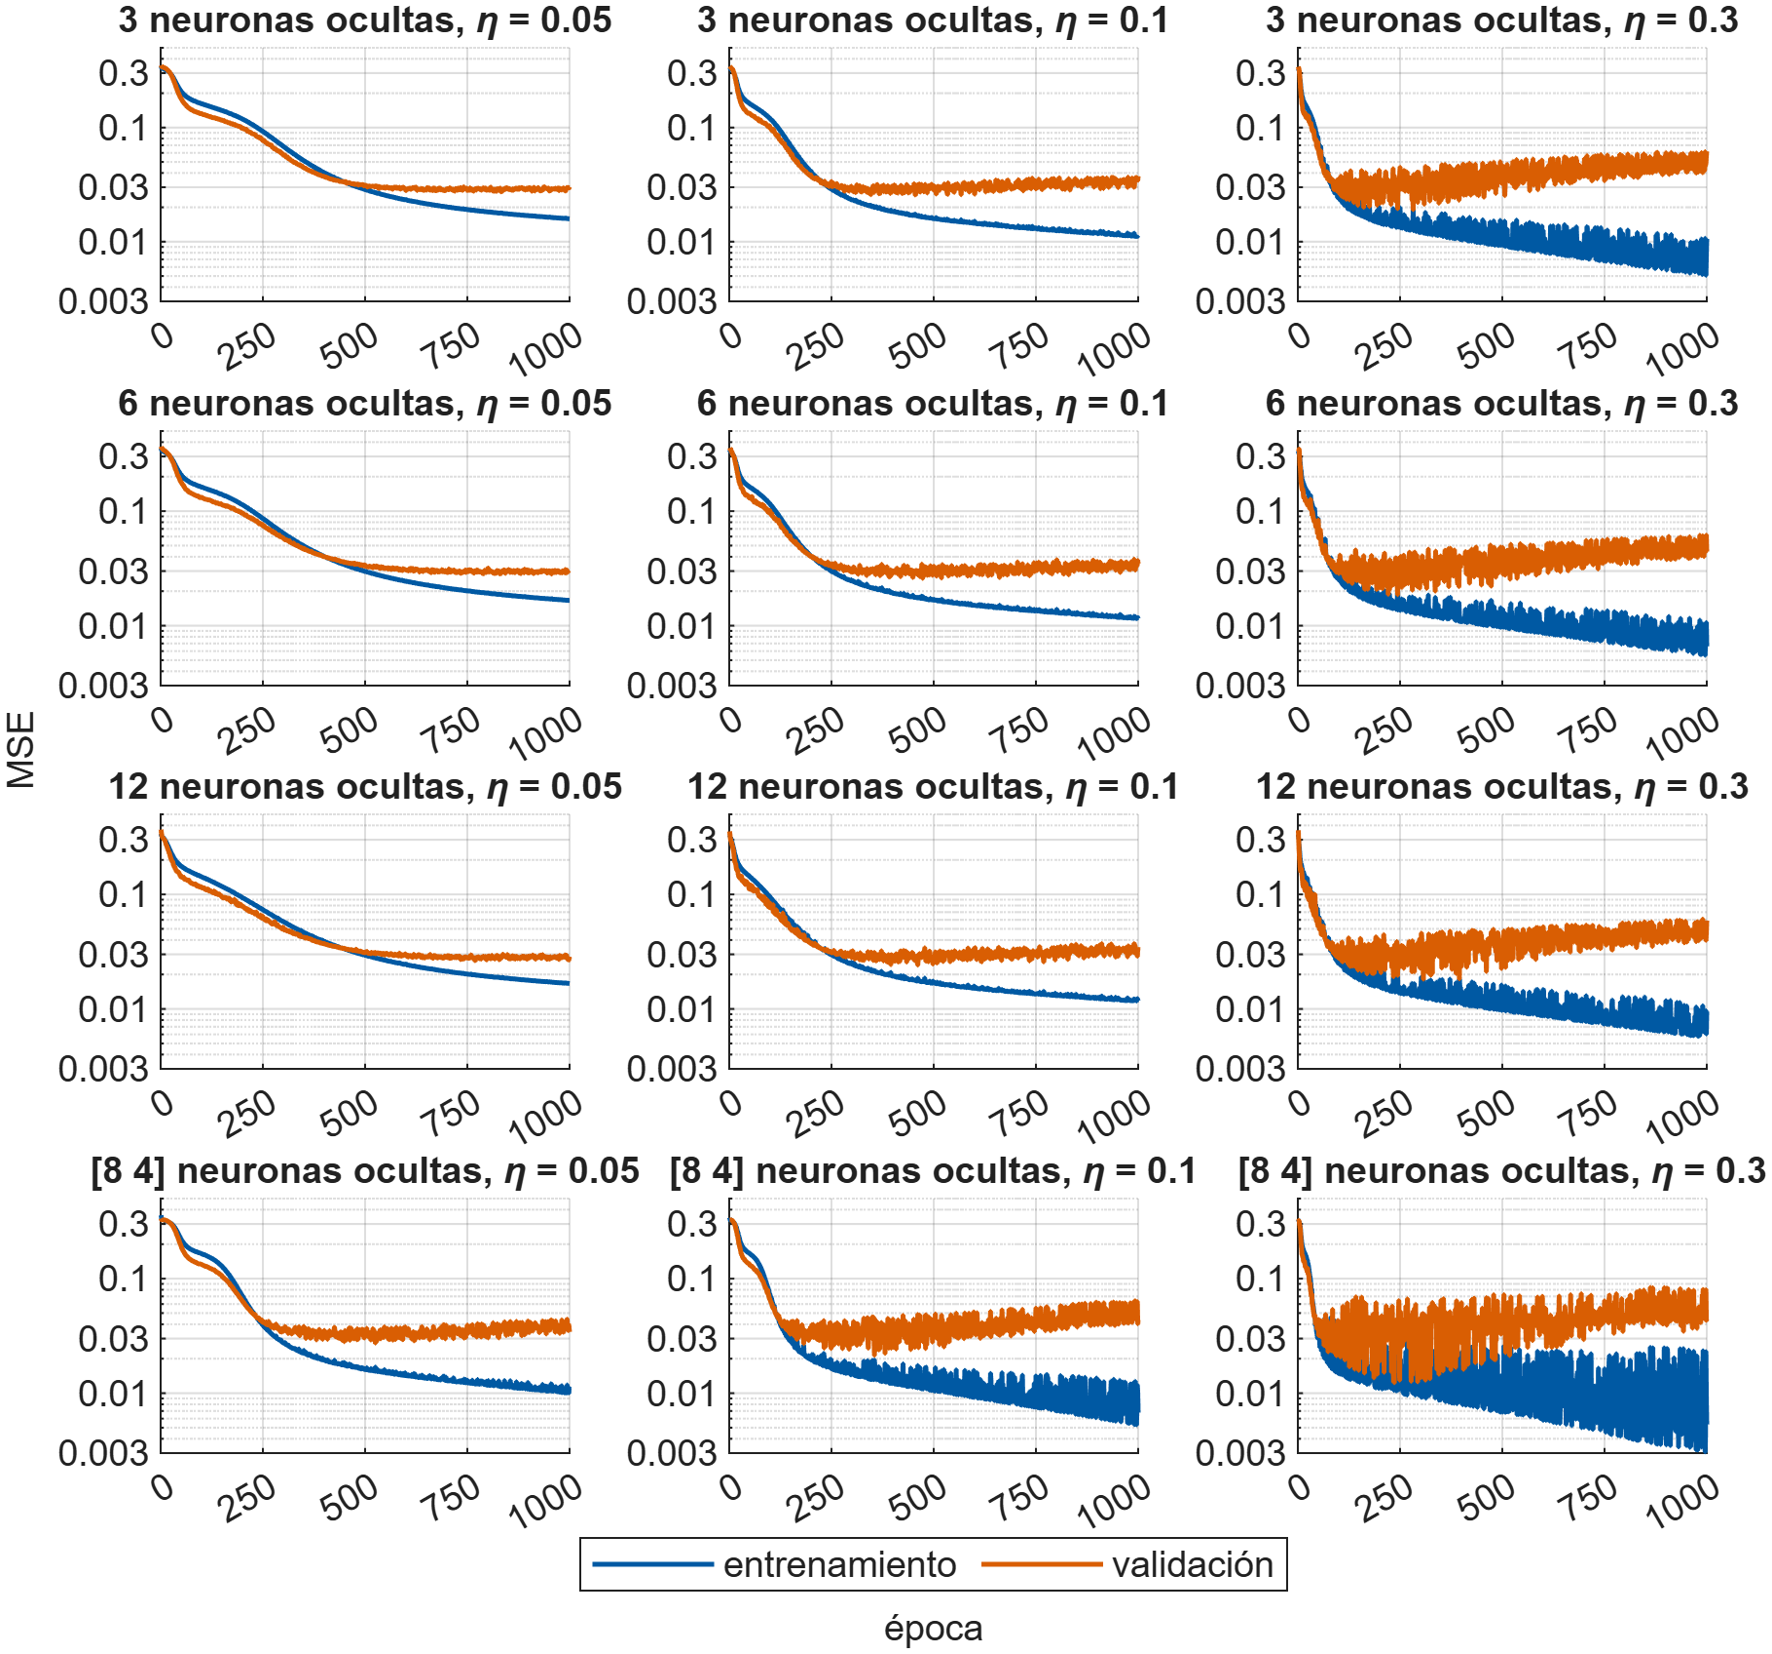
\includegraphics[width=15cm]{fig04.png}
    \caption{Curvas de error de entrenamiento y de validación sobre Iris para las cuatro arquitecturas y las tres tasas de aprendizaje, en escala logarítmica}
    \label{fig:iris}
\end{figure}

\subsection{Wine, Breast Cancer Wisconsin y billetes en distintas particiones}

La Tabla \ref{tab:particiones} y la Figura \ref{fig:particiones} comparan los tres modelos sobre los tres conjuntos y las cuatro proporciones. Billetes se agregó por ser el conjunto del Taller 1. Sus cifras de Perceptrón y Adaline quedan cerca de las de allí sin coincidir, porque el escalado usa las cotas del entrenamiento sin la parte de validación y el orden de los patrones cambia.

\begin{table}[!htb]
    \centering
    \caption{Exactitud de prueba según proporción de partición, con las épocas y el tiempo de entrenamiento en segundos. El MLP usa ocho neuronas ocultas y para por 30 épocas sin mejora en validación o por error objetivo, y sus épocas son las del mejor punto de validación o las de llegada al error objetivo. Las 200 épocas del Adaline en los tres conjuntos y las 100 del Perceptrón en Breast Cancer y billetes son el tope, sin convergencia. Los tiempos cambian ligeramente en cada ejecución}
    \label{tab:particiones}
    \footnotesize
    \begin{tabular}{ll S[table-format=3.1] S[table-format=3.0] S[table-format=1.3] S[table-format=3.1] S[table-format=3.0] S[table-format=1.3] S[table-format=3.1] S[table-format=3.0] S[table-format=1.3]}
        \toprule
         & & \multicolumn{3}{c}{\textbf{MLP}} & \multicolumn{3}{c}{\textbf{Perceptrón}} & \multicolumn{3}{c}{\textbf{Adaline}} \\
        \cmidrule(lr){3-5} \cmidrule(lr){6-8} \cmidrule(lr){9-11}
        \textbf{Conjunto} & \textbf{Partición} & {\textbf{\%}} & {\textbf{Épocas}} & {\textbf{s}} & {\textbf{\%}} & {\textbf{Épocas}} & {\textbf{s}} & {\textbf{\%}} & {\textbf{Épocas}} & {\textbf{s}} \\
        \midrule
        \multirow{4}{*}{Wine}           & 60-40 & 98.6 & 119 & 0.753 & 95.8 & 52 & 0.018 & 97.2 & 200 & 0.070 \\
                                        & 70-30 & 98.1 & 150 & 0.611 & 92.5 & 32 & 0.004 & 96.2 & 200 & 0.016 \\
                                        & 80-20 & 100.0 & 118 & 0.507 & 94.4 & 25 & 0.005 & 97.2 & 200 & 0.019 \\
                                        & 90-10 & 94.4 & 121 & 0.681 & 100.0 & 35 & 0.003 & 94.4 & 200 & 0.023 \\
        \midrule
        \multirow{4}{*}{Breast Cancer}  & 60-40 & 97.4 & 52 & 0.639 & 96.1 & 100 & 0.009 & 95.2 & 200 & 0.018 \\
                                        & 70-30 & 97.7 & 64 & 0.822 & 95.3 & 100 & 0.010 & 97.1 & 200 & 0.018 \\
                                        & 80-20 & 95.6 & 72 & 1.203 & 93.0 & 100 & 0.020 & 96.5 & 200 & 0.021 \\
                                        & 90-10 & 98.2 & 88 & 1.666 & 98.2 & 100 & 0.013 & 98.2 & 200 & 0.022 \\
        \midrule
        \multirow{4}{*}{Billetes}       & 60-40 & 99.5 & 132 & 2.522 & 96.9 & 100 & 0.022 & 96.5 & 200 & 0.031 \\
                                        & 70-30 & 100.0 & 146 & 2.964 & 99.0 & 100 & 0.022 & 95.9 & 200 & 0.037 \\
                                        & 80-20 & 99.3 & 125 & 2.934 & 96.7 & 100 & 0.028 & 96.4 & 200 & 0.044 \\
                                        & 90-10 & 98.5 & 105 & 3.146 & 97.8 & 100 & 0.027 & 95.6 & 200 & 0.054 \\
        \bottomrule
    \end{tabular}
\end{table}

\begin{figure}[!htb]
    \centering
    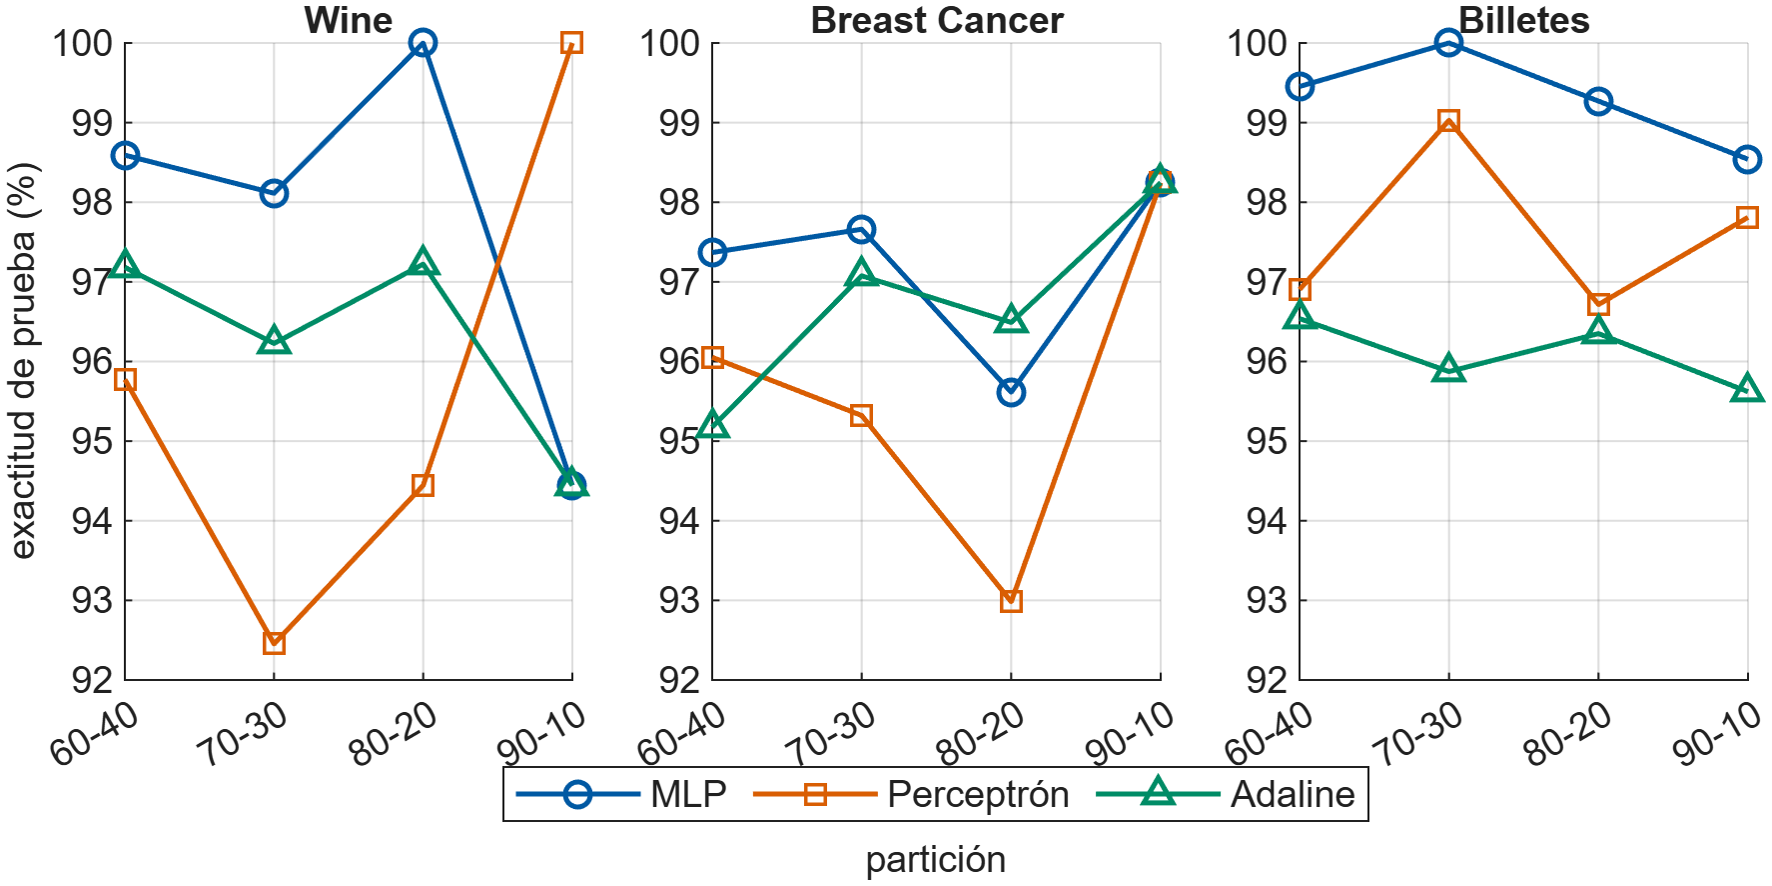
\includegraphics[width=15cm]{fig05.png}
    \caption{Exactitud de prueba de los tres modelos según la proporción de partición en los tres conjuntos reales, con el mismo rango vertical en los tres paneles. En 90-10 los marcadores coinciden donde los modelos empatan}
    \label{fig:particiones}
\end{figure}

En Wine el Perceptrón converge en todas las particiones entre 25 y 52 épocas y aun así el MLP lo supera en tres de cuatro. El Perceptrón se detiene en el primer hiperplano que separa el entrenamiento, por cerca que quede de los patrones, mientras el MLP sigue reduciendo el error hasta que la validación deja de mejorar. La excepción es 90-10, donde el Perceptrón acierta los 18 vinos y el MLP falla uno.

En Breast Cancer el Perceptrón nunca converge en 100 épocas, señal de clases traslapadas. El MLP lo supera en las tres primeras particiones y lo iguala en 90-10, y frente al Adaline solo pierde en 80-20 por un tumor de 114. En billetes la ventaja del MLP es consistente, entre 98.5 y 100 por ciento frente a un máximo de 99.0 del Perceptrón y 96.5 del Adaline. El Adaline queda en medio en Wine y último en billetes, porque el hiperplano que minimiza el error cuadrático no es el que mejor separa las clases.

El costo es el tiempo. El MLP tarda entre 0.507 y 3.146 segundos por entrenamiento contra menos de 0.1 del Perceptrón y el Adaline, entre 10 y 230 veces más según la partición, porque cada patrón atraviesa dos capas en cada sentido y la red evalúa la validación en cada época. En Wine y Breast Cancer el mejor punto de validación llega entre las épocas 52 y 150 y la parada 30 después. En billetes el MLP no usa la parada temprana, porque baja del error objetivo entre las épocas 105 y 146. El Adaline agota sus 200 épocas en los tres conjuntos y el Perceptrón sus 100 en Breast Cancer y billetes, así que ahí sus épocas y su tiempo son los del tope.

\subsection{Análisis de sobreajuste (overfitting)}

La Figura \ref{fig:sobreajuste} muestra ambos errores sobre Breast Cancer durante 1500 épocas para cuatro números de neuronas ocultas, sin parada temprana, y la Tabla \ref{tab:sobreajuste} resume las cifras. Las cuatro curvas tienen la misma forma. El error de validación toca un mínimo entre 0.0068 y 0.0079 entre las épocas 85 y 165 y después sube hasta terminar entre 0.0187 y 0.0220, casi el triple, mientras el de entrenamiento sigue bajando hasta 0.0036. Esa separación creciente es el sobreajuste.

\begin{figure}[!htb]
    \centering
    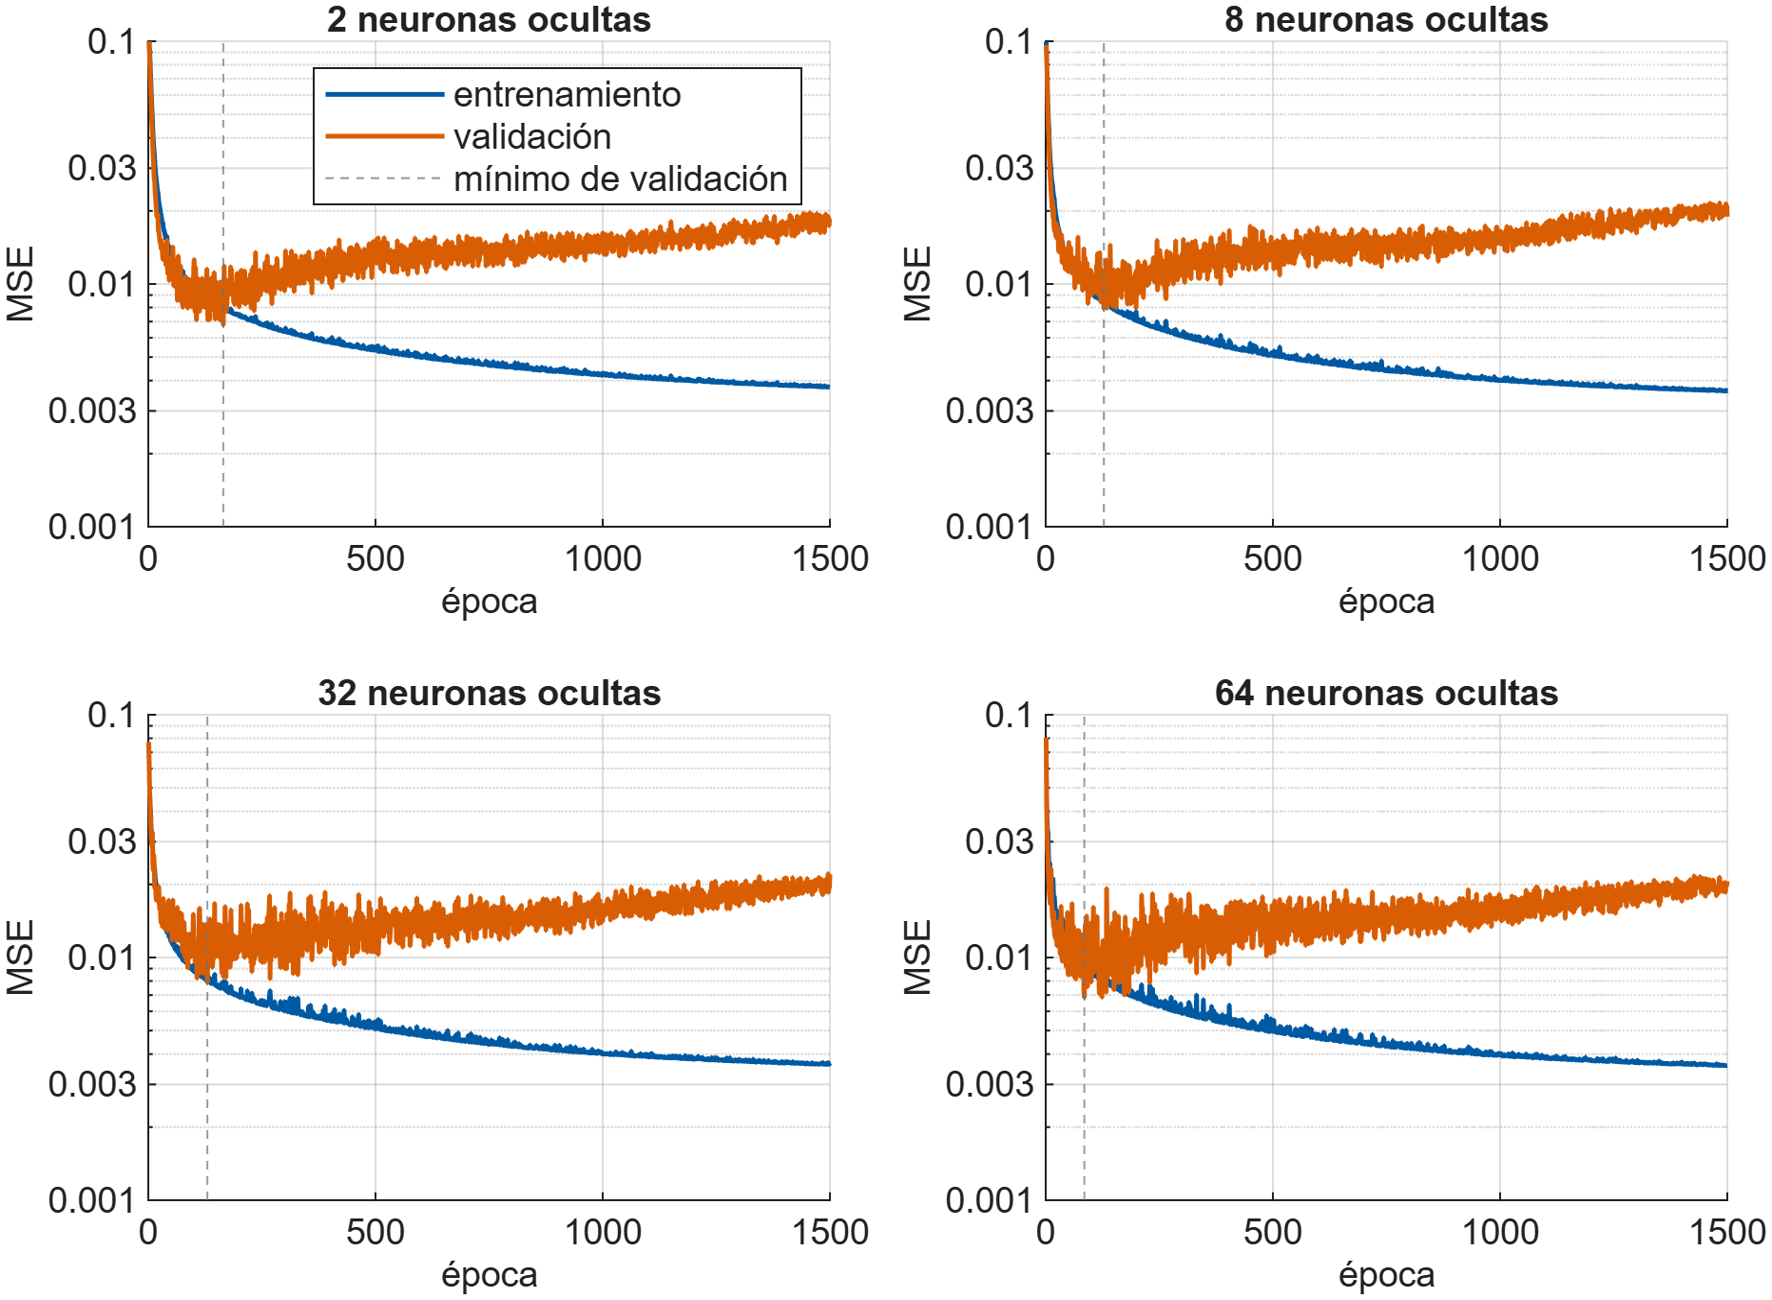
\includegraphics[width=15cm]{fig06.png}
    \caption{Error de entrenamiento y de validación sobre Breast Cancer para cuatro números de neuronas ocultas. La línea discontinua marca la época de mínimo error de validación. Escala logarítmica}
    \label{fig:sobreajuste}
\end{figure}

\begin{table}[!htb]
    \centering
    \caption{Sobreajuste en Breast Cancer, partición 70-30. Sin parada temprana el entrenamiento dura 1500 épocas, con parada temprana se detiene tras 50 épocas sin mejora en validación}
    \label{tab:sobreajuste}
    \scriptsize
    \begin{tabular}{c S[table-format=1.4] S[table-format=1.4] S[table-format=3.0] S[table-format=1.4] S[table-format=2.1] S[table-format=3.0] S[table-format=2.1]}
        \toprule
         & \multicolumn{5}{c}{\textbf{Sin parada temprana, 1500 épocas}} & \multicolumn{2}{c}{\textbf{Con parada temprana}} \\
        \cmidrule(lr){2-6} \cmidrule(lr){7-8}
        \textbf{Ocultas} & {\textbf{MSE ent.}} & {\textbf{MSE val.}} & {\textbf{Época mín.}} & {\textbf{MSE val. mín.}} & {\textbf{Exact. (\%)}} & {\textbf{Épocas}} & {\textbf{Exact. (\%)}} \\
        \midrule
        2  & 0.0038 & 0.0187 & 165 & 0.0068 & 94.7 & 215 & 97.7 \\
        8  & 0.0036 & 0.0189 & 128 & 0.0079 & 94.7 & 178 & 97.7 \\
        32 & 0.0037 & 0.0220 & 130 & 0.0079 & 94.2 & 180 & 97.7 \\
        64 & 0.0036 & 0.0206 & 85  & 0.0068 & 94.7 & 135 & 97.7 \\
        \bottomrule
    \end{tabular}
\end{table}

La Tabla \ref{tab:epocas} aísla el efecto del número de épocas con ocho neuronas ocultas. Cada entrenamiento más largo baja el error de entrenamiento y sube el de validación, y la exactitud de prueba cae de 95.9 por ciento a las 200 épocas a 94.7 a las 1000 y 1500, es decir dos tumores más mal clasificados por seguir entrenando.

\begin{table}[!htb]
    \centering
    \caption{Efecto del número de épocas con ocho neuronas ocultas sobre Breast Cancer, sin parada temprana}
    \label{tab:epocas}
    \footnotesize
    \begin{tabular}{S[table-format=4.0] S[table-format=1.4] S[table-format=1.4] S[table-format=2.1]}
        \toprule
        {\textbf{Épocas}} & {\textbf{MSE entrenamiento}} & {\textbf{MSE validación}} & {\textbf{Exactitud de prueba (\%)}} \\
        \midrule
        200  & 0.0071 & 0.0115 & 95.9 \\
        500  & 0.0051 & 0.0126 & 95.3 \\
        1000 & 0.0040 & 0.0146 & 94.7 \\
        1500 & 0.0036 & 0.0189 & 94.7 \\
        \bottomrule
    \end{tabular}
\end{table}

La parada temprana guarda los pesos del mejor punto y detiene el entrenamiento tras 50 épocas sin mejorar el mínimo de validación. Termina entre las épocas 135 y 215 y la exactitud de prueba sube a 97.7 por ciento en los cuatro casos, cuatro tumores fallados de 171, frente a 94.2 a 94.7 sin parada. El número de neuronas apenas cambia el resultado. Con 2 y con 64 el mínimo de validación vale lo mismo, la red grande solo llega antes.

% ============================================================
\section{Análisis y discusión}

\subsection{Por qué el MLP resuelve la XOR y los modelos del Taller 1 no}

El Perceptrón y el Adaline quedan en 30 y cerca de 50 por ciento porque una neurona traza un hiperplano y ninguno separa la XOR. El MLP transforma la entrada antes de decidir. Cada neurona oculta traza su hiperplano y la salida combina las regiones, así que el problema que llega a la salida ya es separable. La fila de dos neuronas confirma que dos rectas bastan, pues clasifica bien en las cinco semillas aunque una no baje el error por debajo de 0.001. Con cuatro u ocho sobran neuronas para trazarlas y todas las semillas llegan al objetivo.

Con tres entradas hay ocho vértices de un cubo alternando clase y hacen falta más regiones. El momento fue decisivo. Con $\beta$ 0.9 la corrección acumula impulso en la dirección que se repite época tras época y atraviesa las mesetas donde el gradiente es pequeño, los tramos planos de la curva de tres entradas en la Figura \ref{fig:xor}.

\subsection{Efecto del número de neuronas ocultas y de la tasa de aprendizaje}

Un valor pequeño de tasa da curvas suaves pero lentas, como 0.05 en Iris, que a las 1000 épocas no se ha estabilizado. Un valor grande llega antes pero oscila, como 0.3 en la Figura \ref{fig:iris}, donde el error de validación se despega del de entrenamiento.

El número de neuronas ocultas importó menos de lo esperado. En Iris las cuatro arquitecturas dan la misma exactitud con 0.1 y 0.3, y en Breast Cancer los cuatro tamaños caen en un mínimo de validación muy parecido, entre 0.0068 y 0.0079. Solo en la XOR, donde la geometría exige un número mínimo de hiperplanos, el tamaño decide entre converger o no. En los conjuntos reales las neuronas adicionales no mejoran la clasificación, solo agregan pesos, y en la Tabla \ref{tab:iris} el tiempo crece poco entre tres y doce neuronas y da un salto con la segunda capa.

\subsection{Proporción de partición y generalización}
\label{sec:particiones}

Con una semilla por partición, ninguna proporción resultó mejor de forma consistente. En Wine el Perceptrón alcanza su máximo en 90-10 y el MLP en 80-20, en Breast Cancer el MLP se mueve entre 95.6 y 98.2 sin orden, y en billetes las cuatro dan entre 98.5 y 100. Lo que sí se repite es la fragilidad de las pruebas pequeñas. Con 18 vinos o 57 tumores un solo error mueve la exactitud entre 1.8 y 5.6 puntos, y por eso el 100 por ciento del Perceptrón en Wine 90-10 o del MLP en Wine 80-20 dicen menos de lo que parecen.

\subsection{Evidencia de sobreajuste y su mitigación}

La evidencia está en la Figura \ref{fig:sobreajuste} y en la Tabla \ref{tab:epocas}. A las 1500 épocas la red clasifica peor que a las 200, 1.2 puntos menos, y entre 3.0 y 3.5 puntos menos que la red detenida a tiempo, aunque su error sobre los datos ya vistos sea cinco veces menor que el de validación.

La parada temprana lo corrigió en los cuatro casos y los llevó al mismo 97.7 por ciento, sin decidir de antemano el número de épocas, porque lo decide la validación. El precio es apartar datos, aquí 80 de 398, con lo cual la red aprende con menos ejemplos pero la prueba mide lo que la red no vio. Subir de 2 a 64 neuronas no agravó el sobreajuste, solo lo adelantó de la época 165 a la 85. La causa aquí es el exceso de épocas y el remedio es parar a tiempo, no reducir la red.

% ============================================================
\section{Conclusiones}

El perceptrón multicapa resolvió la XOR de dos entradas al 100 por ciento en todas las semillas con cuatro u ocho neuronas ocultas, y la de tres entradas al agregar momento 0.9. El Perceptrón y el Adaline, con los parámetros del Taller 1, quedaron en promedio en 30 por ciento con dos entradas y entre 47.5 y 50 con tres. Dos neuronas ocultas bastan para clasificar, aunque con ellas una de cinco semillas no llega al error objetivo.

El momento fue el parámetro de mayor efecto sobre la velocidad. Con 0.9 la XOR de dos entradas pasó de 4117 a 436 épocas y la de tres de dos semillas convergidas a cinco. El barrido de la guía mostró que la tasa llega a 2 sin desestabilizar, que el momento 1 impide converger y que la escala inicial solo lleva todas las semillas al objetivo entre 0.5 y 2. Entre las activaciones, la salida sigmoide convergió con cualquier capa oculta, mientras que la salida tanh o lineal sobre una oculta tanh hizo oscilar la red con momento 0.9.

Sobre Iris las doce configuraciones dieron 95.6 o 97.8 por ciento, y la tasa determinó la forma de la curva más que el número de neuronas o de capas. Por error de validación la mejor fue doce neuronas con tasa 0.05, y por estabilidad la tasa 0.1. Sobre 45 flores ninguna se distingue por exactitud.

En los conjuntos reales el MLP superó al Perceptrón en diez de las doce particiones y al Adaline en nueve, y solo perdió dos veces, en Wine 90-10 frente al Perceptrón y en Breast Cancer 80-20 frente al Adaline, cada vez por un solo patrón de prueba. La ventaja más clara estuvo en billetes, entre 98.5 y 100 por ciento. El precio fue un tiempo de entrenamiento entre 10 y 230 veces mayor.

El sobreajuste apareció en Breast Cancer como una subida sostenida del error de validación desde las épocas 85 a 165 mientras el de entrenamiento seguía bajando. Costó 1.2 puntos de exactitud entre 200 y 1500 épocas, y su magnitud no dependió del número de neuronas ocultas entre 2 y 64, aunque la red más grande llegó antes al mínimo. La parada temprana por 50 épocas sin mejora lo corrigió y elevó la exactitud de prueba de entre 94.2 y 94.7 a 97.7 por ciento en los cuatro casos.

Ninguna proporción de partición resultó mejor de forma consistente. Las particiones 90-10 evalúan sobre muy pocos patrones, y el 100 por ciento del Perceptrón en Wine 90-10 equivale a un vino más acertado que el MLP.

% ============================================================
\section{Referencias}
\begin{itemize}
    \item Rumelhart, D. E., Hinton, G. E., \& Williams, R. J. (1986). Learning representations by back-propagating errors. \textit{Nature}, 323(6088), 533--536.
    \item Haykin, S. (2009). \textit{Neural Networks and Learning Machines} (3.\textsuperscript{a} ed.). Pearson.
    \item Redes neuronales, algoritmo Backpropagation (2007). Guía de laboratorio, material del curso Inteligencia Computacional Aplicada, Universidad Distrital Francisco José de Caldas.
    \item Fisher, R. A. (1936). The use of multiple measurements in taxonomic problems. \textit{Annals of Eugenics}, 7(2), 179--188.
    \item Aeberhard, S., \& Forina, M. (1991). Wine. UCI Machine Learning Repository.
    \item Wolberg, W., Mangasarian, O., Street, N., \& Street, W. (1993). Breast Cancer Wisconsin (Diagnostic). UCI Machine Learning Repository.
    \item Lohweg, V. (2013). Banknote Authentication. UCI Machine Learning Repository.
\end{itemize}

% ============================================================
\appendix
\section{Tablas complementarias}
\label{anexo:tablas}

\begin{table}[!htb]
    \centering
    \caption{Matrices de confusión de las doce configuraciones sobre Iris. Cada celda es el número de flores de la clase real en fila asignadas a la clase en columna, con las clases en el orden setosa, versicolor, virginica}
    \label{tab:iris_todas}
    \footnotesize
    \begin{tabular}{c S[table-format=1.2] *{9}{S[table-format=2.0]}}
        \toprule
        \textbf{Ocultas} & {$\boldsymbol{\eta}$} & {\textbf{se-se}} & {\textbf{se-ve}} & {\textbf{se-vi}} & {\textbf{ve-se}} & {\textbf{ve-ve}} & {\textbf{ve-vi}} & {\textbf{vi-se}} & {\textbf{vi-ve}} & {\textbf{vi-vi}} \\
        \midrule
        3     & 0.05 & 14 & 0 & 0 & 0 & 11 & 2 & 0 & 0 & 18 \\
        3     & 0.1  & 14 & 0 & 0 & 0 & 12 & 1 & 0 & 0 & 18 \\
        3     & 0.3  & 14 & 0 & 0 & 0 & 12 & 1 & 0 & 0 & 18 \\
        6     & 0.05 & 14 & 0 & 0 & 0 & 11 & 2 & 0 & 0 & 18 \\
        6     & 0.1  & 14 & 0 & 0 & 0 & 12 & 1 & 0 & 0 & 18 \\
        6     & 0.3  & 14 & 0 & 0 & 0 & 12 & 1 & 0 & 0 & 18 \\
        12    & 0.05 & 14 & 0 & 0 & 0 & 11 & 2 & 0 & 0 & 18 \\
        12    & 0.1  & 14 & 0 & 0 & 0 & 12 & 1 & 0 & 0 & 18 \\
        12    & 0.3  & 14 & 0 & 0 & 0 & 12 & 1 & 0 & 0 & 18 \\
        {[8 4]} & 0.05 & 14 & 0 & 0 & 0 & 12 & 1 & 0 & 0 & 18 \\
        {[8 4]} & 0.1  & 14 & 0 & 0 & 0 & 12 & 1 & 0 & 0 & 18 \\
        {[8 4]} & 0.3  & 14 & 0 & 0 & 0 & 12 & 1 & 0 & 0 & 18 \\
        \bottomrule
    \end{tabular}
\end{table}

\lstset{basicstyle=\ttfamily\scriptsize}
\section{Código de los bloques completados}
\label{anexo:codigo}

Se reproducen completos los cuatro bloques que la plantilla dejaba pendientes y la función de entrenamiento con parada temprana que se agregó para los experimentos. Ningún nombre ni argumento de las funciones de la plantilla fue modificado.

\noindent\begin{minipage}{\linewidth}
\lstinputlisting[language=Matlab,caption={Inicialización de pesos y sesgos}]{fragmentos/init_mlp.m}
\end{minipage}
\vspace{0.6em}

\noindent\begin{minipage}{\linewidth}
\lstinputlisting[language=Matlab,caption={Propagación hacia adelante}]{fragmentos/forward_mlp.m}
\end{minipage}
\vspace{0.6em}

\noindent\begin{minipage}{\linewidth}
\lstinputlisting[language=Matlab,caption={Retropropagación del error y actualización con momento}]{fragmentos/backward_mlp.m}
\end{minipage}
\vspace{0.6em}

\noindent\begin{minipage}{\linewidth}
\lstinputlisting[language=Matlab,caption={Derivadas de las funciones de activación}]{fragmentos/activation_deriv.m}
\end{minipage}
\vspace{0.6em}

\noindent\begin{minipage}{\linewidth}
\lstinputlisting[language=Matlab,caption={Entrenamiento con error de validación y parada por épocas sin mejora}]{fragmentos/train_mlp.m}
\end{minipage}

\end{document}
